% Preamble
\documentclass[11pt]{article}

% Packages
\usepackage{amsmath}
\usepackage{tikz}
\usepackage{color}
\usepackage{xcolor}
\usetikzlibrary{arrows}
\tikzset{
    >=stealth' % Default arrow tip
    %    node distance=2.8cm
}

\tikzstyle{vertex}=[
    draw,
    circle,
    fill = black,
    inner sep = 0cm,
    minimum width = 0.12cm
]

\tikzstyle{weight}=[fill=white]

\newcommand{\CYAN}[1]{\textcolor{cyan}{#1}}
\newcommand{\ORNG}[1]{\textcolor{orange}{#1}}

% Document
\begin{document}

\section[V]{Vector}

\subsection{Vector types}

\subsubsection{Zero vector}

Vector containing only zeroes.

$$
\vec{o} = \begin{bmatrix}0 & 0\end{bmatrix}
$$

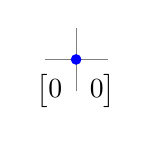
\begin{tikzpicture}
    \draw [gray, very thin] (-0.4, -0.4) grid (0.4, 0.4);

    \draw node [vertex, blue, label=below:$\begin{bmatrix}0 & 0\end{bmatrix}$] (1) at (0, 0) {};
\end{tikzpicture}


\subsubsection{Inverse vector}

Each vector $\vec{\Green v}$ has an inverse vector $-\vec{\Green v}$

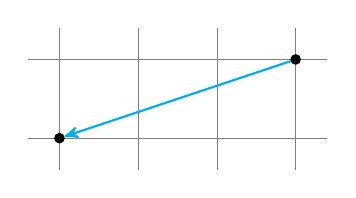
\begin{tikzpicture}
    \draw [gray, very thin] (-0.4, -0.4) grid (3.4, 1.4);

    \draw node [vertex] (1) at (0, 0) {};
    \draw node [vertex] (2) at (3, 1) {};

    \draw [thick, cyan, ->] (2) -- (1);
\end{tikzpicture}


\subsection{Vector operations}
\subsubsection{Vector addition}

$$
\CYAN{\vec{v}} + \ORNG{\vec{w}} = \begin{bmatrix}
    \CYAN{v_1} \\ \CYAN{v_2}
\end{bmatrix} + \begin{bmatrix}
    \ORNG{w_1} \\ \ORNG{w_2}
\end{bmatrix} = \begin{bmatrix}
    \CYAN{v_1} + \ORNG{w_1} \\ \CYAN{v_2} + \ORNG{w_2}
\end{bmatrix}
$$

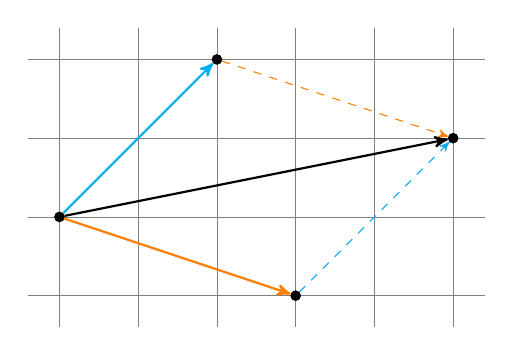
\begin{tikzpicture}
    \draw [gray, very thin] (-0.4, -1.4) grid (5.4, 2.4);

    \draw node [vertex] (o) at (0, 0) {};
    \draw node [vertex] (v) at (2, 2) {};
    \draw node [vertex] (w) at (3, -1) {};
    \draw node [vertex] (r) at (5, 1) {};

    \draw [thick, cyan, ->] (o) -- (v);
    \draw [thick, orange, ->] (o) -- (w);
    \draw [orange, dashed, ->] (v) -- (r);
    \draw [cyan, dashed, ->] (w) -- (r);
    \draw [thick, ->] (o) -- (r);
\end{tikzpicture}

\end{document}
